\chapter{Introducción} % (fold)
\label{cha:introduccion}

El presente proyecto consiste en el desarrollo de una aplicación móvil que permita ubicar y encontrar una locación dentro del campus de la Universidad Mayor de San Simón, la aplicación deberá localizar la ubicación actual del usuario y permitir especificar un punto de destino, mostrando a continuación el camino más corto para llegar a destino.

El campus universitario abarca más de 214,000 $m^2$ y encierra varias facultades y oficinas administrativas, para estudiantes nuevos y antiguos o personas que
necesitan hacer trámites administrativos, incluso si solo se quiere conocer el
campus, es necesario contar con un mapa donde ubicarse.

Las aplicaciones móviles tienen una gran demanda por parte de la población ya
que la gran mayoría posee un \emph{smartphone} o teléfono inteligente con capacidad de
ejecutar aplicaciones muy fácilmente, los \emph{smartphones} cuentan también con GPS,
el cual se usa para conocer la ubicación del usuario con un margen de error de
3 metros, usando puntos de referencia geo-localizados se puede determinar la
ruta óptima para llegar a destino. Es una desventaja para nuestra Universidad que no exista información confiable de fácil acceso para poder desplazarse por el campus.

  \section{Antecedentes} % (fold)
  \label{sec:antecedentes}

  Actualmente \emph{Google Maps} ofrece una solución al problema de encontrar una ruta entre 2 puntos geolocalizados, ya que sugiere posibles rutas si se usara movilidad, bicicleta o para ir caminando, para lograr esto se toman en cuenta los distintos tipos de calles que existen y la dirección en el caso de movilidades, \emph{Google Maps} toma en cuenta la descripción de una locación o la referencia cartográfica en latitud y longitud de los puntos, y el cómo se va a desplazar entre los 2 puntos para dibujar con una línea roja la ruta a seguir.

  Así como también existen Blogs o Aplicaciones con información de los lugares turísticos o de interés para visitar en la ciudad, como ser TripAdvisor, la información que provee esta aplicación generalmente incluye la locación del lugar referenciada sobre un mapa estático, este tipo de aplicaciones usa el API de \emph{Google Maps} para lograr encontrar una ruta hacia el lugar de interés.

  En el caso del campus de la Universidad Mayor de San Simón, Google Maps no cuenta con la información para lograr este objetivo, de encontrar una ruta entre 2 puntos geo-referenciados, ya que se necesita de un mapa de los caminos internos del campus Universitario e información de las aulas, kioscos, fotocopiadoras, oficinas, etc. Esta información no está disponible o es de difícil acceso lo cual genera malestar cuando se busca una locación dentro del campus Universitario.

  \section{Descripción del problema} % (fold)
  \label{sec:desc_probl}

  % Al andar dentro del campus universitario buscando algún lugar o punto de interés, es generalmente de gran prioridad reducir el tiempo en el cual se llega al aula u oficina, lamentablemente el campus Universitario carece de un buen sistema de señalización por lo que para llegar al punto de destino es necesario preguntar la  la Universidad hacia gente externa que necesitan hacer uso o encontrar algún lugar en especifico ya que lamentablemente esta información actualmente sólo te la pueden ofrecer las personas que conocen el lugar de antemano y aun en esos casos existe la posibilidad de no encontrar el lugar que se está buscando.\\

  La Universidad Mayor de San Simón no cuenta con un mapa interactivo que
  muestre la ubicación de los puntos o lugares que se encuentran dentro del
  campus universitario y como llegar hasta su ubicación, la falta de señalización obstaculiza el desplazamiento de los estudiantes o personas que requieren encontrar alguna oficina para, por ejemplo, realizar trámites administrativos, encontrar aulas o auditorios, etc. como resultado se pierde tiempo al tratar de encontrarlos por lo que un mapa con estas características sería de gran ayuda para el desplazamiento dentro del campus universitario. En la figura  \ref{fig:arbolProblemas}, se puede apreciar al árbol de problemas.

  % \begin{figure}[!hbp]
  %   \centering
  %   \includesvg{arbolProblemas}
  %   \caption{Diagrama Árbol de Problemas}
  %   \label{fig:arbolProblemas}
  % \end{figure}


  \begin{figure}[!ht]
    \begin{center}
      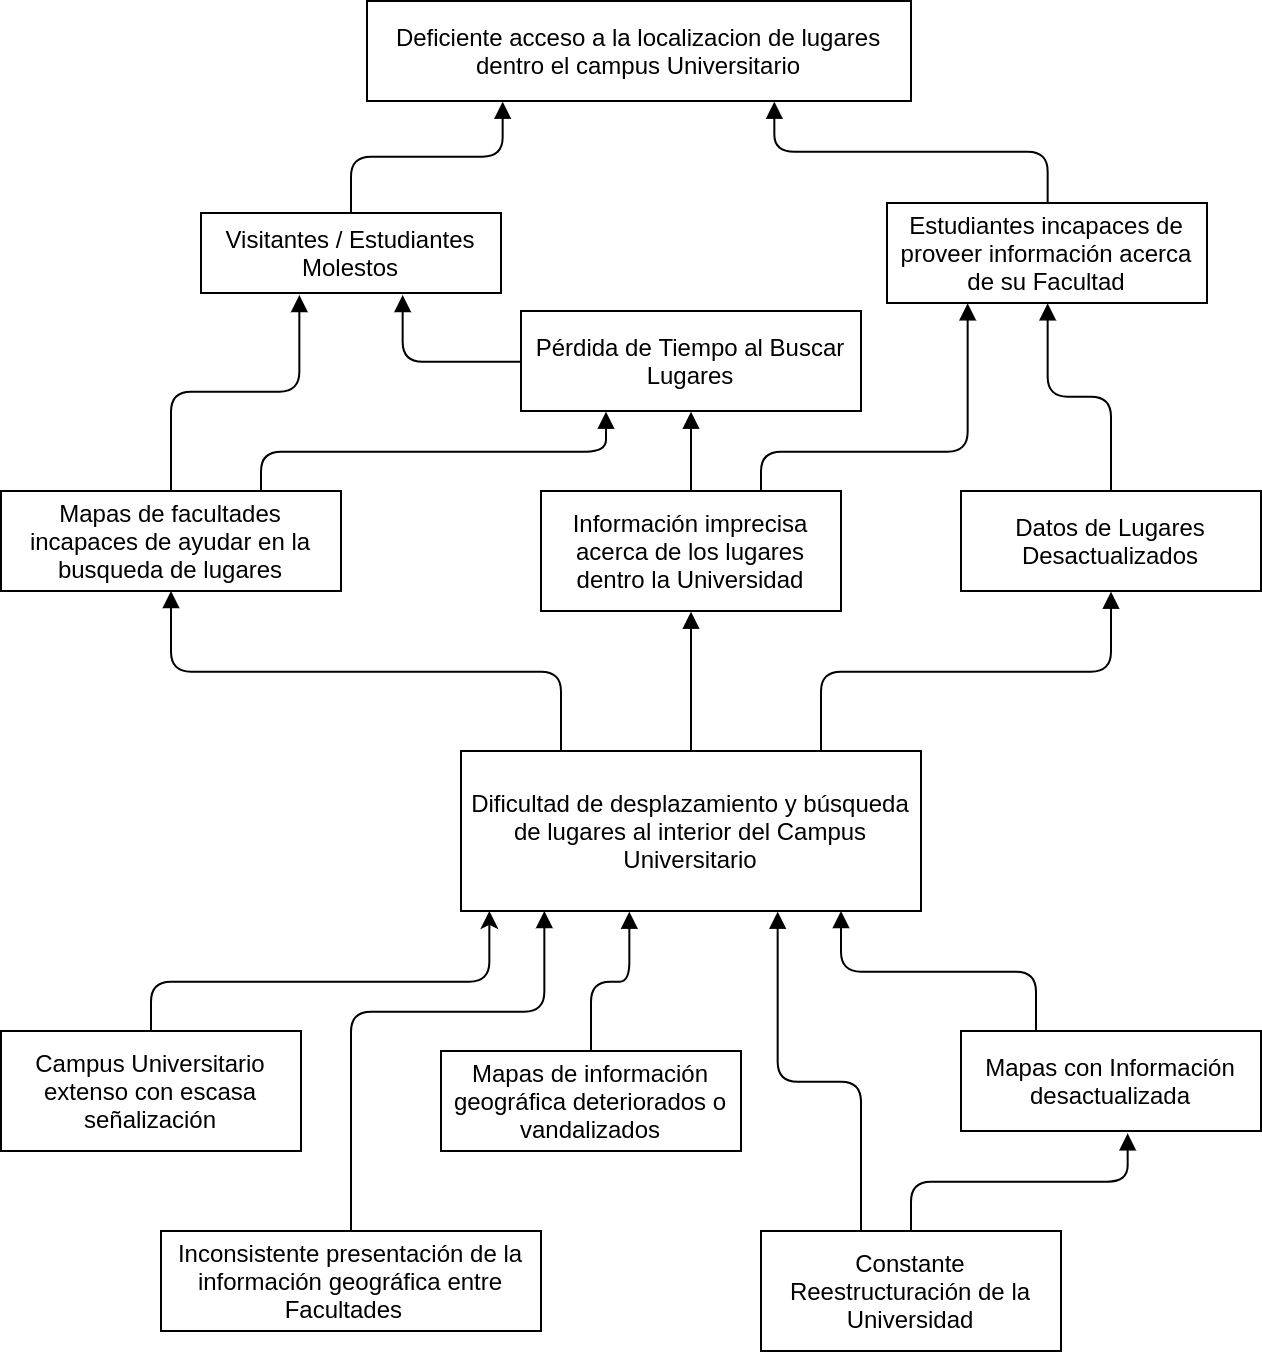
\includegraphics[width=0.65\textwidth]{diagramas/arbolProblemas}
    \end{center}
    \caption{Diagrama Árbol de Problemas}
    \label{fig:arbolProblemas}
    \caption*{Fuente: Elaboración propia}
  \end{figure}

  \section{Objetivo general} % (fold)
  \label{sec:objetivo_general}
    \begin{quote}
      Desarrollar una aplicación web móvil \emph{responsiva} para optimizar la búsqueda de lugares y el  desplazamiento al interior del Campus Universitario de la UMSS.
    \end{quote}
  % section objetivo_general (end)


  \section{Objetivos Específicos} % (fold)
  \label{sec:obj_especificos}
    \begin{itemize}
      \item Generar un mapa con información geográfica de las rutas dentro del campus Universitario.
      \item Administrar lugares geolocalizados dentro del campus Universitario.
      \item Mostrar en la aplicación los lugares geolocalizados desplegando la ruta óptima desde mi posición hasta el punto destino.
      \item Administrar usuarios en el sistema.
      \item Registrar las búsquedas sobre rutas realizadas por los usuarios en el sistema.
    \end{itemize}
  % section obj_especificos (end)


  \section{Justificación} % (fold)
  \label{sec:justificacion}

  El Campus Universitario es bastante extenso y se encuentra en constante reestructuración, debido a que las aulas se incrementan, las oficinas son reubicadas, etc. gracias a esto es que los mapas con los que cuenta cada facultad, que son escasos y están impresos sobre banners estáticos, son también difíciles de actualizar. Este hecho genera malestar en estudiantes que llegan tarde a sus clases o necesitan llegar a algún Auditorio o personas/visitantes en proceso de realizar trámites administrativos, no encuentran con facilidad las oficinas a las que necesitan llegar.

  Una aplicación que permita localizar o encontrar locaciones y además proveer la ruta óptima dentro del campus de la Universidad Mayor de San Simón es de gran importancia para brindar apoyo a cualquier persona que necesite desplazarse por el campus Universitario.

  Las Aplicaciones móviles y/o web demostraron ser el futuro del desarrollo de software y la gran mayoría de los países en el mundo consumen estas soluciones y es necesario apuntar a esta tendencia.


  % section justificacion (end)
% chapter introduccion (end)

  \section{Alcance}
  \label{sec:Alcance}

    \subsection{Alcance Práctico}
    \label{sub:alcance_practico}

    Una aplicación web móvil puede llegar a ser muy compleja y manejar información sensible, y ya que el servidor está expuesto al acceso público de los usuarios, es susceptible de ataques maliciosos y malintencionados para acceder y robar información privada que los usuarios podrían tener almacenados en la aplicación, en el caso de la presente aplicación, el sistema no manejará información sensible del usuario, como ser tarjetas de crédito pero la aplicación manejará información de lugares, información que podría ser corrompida por usuarios malintencionados. La seguridad es muy importante para una aplicación web, por lo cual el presente proyecto implementara medidas de seguridad para asegurar la identidad del usuario que está solicitando el ingreso al sistema pero no incluirá protección a ataques Phishing, DoS ya que los objetivos específicos no los contempla.\\


    El \emph{look and feel} de una aplicación web es un tema muy importante para cualquier aplicación a desarrollar, para lograr que la aplicación se muestre de manera consistente en la pantalla de un smartphone se usarán herramientas de terceros pero no se extenderá el uso de la misma para la pantalla de un ordenador de escritorio que posee una resolución de pantalla muy superior al de un celular.\\



    % end alcance_practico

    \subsection{Alcance Metodológico}
    \label{sub:alcance_metodologico}
    Para la conclusión exitosa del presente proyecto se implementará la metodología  Programación Extrema (XP) y cada iteración del proceso tiene como meta el desarrollo conjunto de diferentes módulos, historias de usuario y la documentación relacionada.
    % end alcance_metodologico

    \subsection{Alcance Teórico}
    \label{sub:alcance_teorico}
    La investigación se limita a las estructuras, herramientas y estándares actuales sugeridos en la documentación y bibliografía consultada para la construcción de una aplicación web móvil.
    % end alcance_teorico

  % end Alcance






% Metodología:
% Agile Unified Process (AUP) es una versión simplificada de Rational  Proceso
% Unificado  (RUP).

% Fases del ciclo de desarrollo
%   Principio: El objetivo es  identificar el alcance inicial del proyecto y una
%   arquitectura potencial del sistema.

%   Elaboración: El objetivo es confirmar la idoneidad de la arquitectura del sistema.
%   Construcción: El objetivo es desarrollar software funcional dentro de un sistema regular e incremental periódicamente que mire las necesidades de las partes interesadas.
%   Transición: El objetivo es validar y desplegar el sistema en su entorno de producción.
% Las disciplinas del ciclo de desarrollo se llevan de manera iterativa y son
% las siguientes
%   Modelo: El objetivo de esta disciplina es entender el negocio de la organización, el dominio del problema que se ocupa el proyecto, y determinar una solución viable para hacer frente al dominio del problema.
%   Aplicación: El objetivo de esta disciplina es transformar el modelo de su (s) en el código ejecutable y para llevar a cabo un nivel básico de las pruebas, en las pruebas de unidad en particular.
%   Prueba: El objetivo de esta disciplina consiste en realizar una evaluación objetiva para asegurar la calidad. Esto incluye encontrar defectos, validar que el sistema funcione como está previsto, y verificar que se cumplan los requisitos.
%   Implementación: El objetivo de esta disciplina es el plan para la entrega del sistema y para ejecutar el plan para que el sistema a disposición de los usuarios finales.
%   Gestión de la Configuración: El objetivo de esta disciplina consiste en administrar el acceso a artefactos de su proyecto. Esto incluye no sólo el seguimiento de versiones de los artefactos a través del tiempo, sino también el control y la gestión de los cambios a los mismos.
%   Gestión de Proyectos: El objetivo de esta disciplina es dirigir las actividades que lleva a cabo en el proyecto. Esto incluye la gestión de riesgos, la dirección de personas (la asignación de tareas, seguimiento de los progresos, etc.), y coordinar con la gente y los sistemas fuera del alcance del proyecto para asegurarse de que se entregue a tiempo y dentro del presupuesto.
%   Para el Medio Ambiente: El objetivo de esta disciplina es apoyar el resto de los esfuerzos por garantizar que el proceso, la orientación adecuada (las normas y directrices), y herramientas (hardware, software, etc.) están disponibles para el equipo según sea necesario.
% % Fig. Ciclo de vida del Proceso Unificado Ágil
